% !TEX TS-program = pdflatex
% !TEX encoding = UTF-8 Unicode

% This is a simple template for a LaTeX document using the "article" class.
% See "book", "report", "letter" for other types of document.

\documentclass[11pt]{article} % use larger type; default would be 10pt


\usepackage{ulem}
\newcommand\NoIndent[1]{%
  \par\vbox{\parbox[t]{\linewidth}{#1}}%
}


\usepackage[utf8]{inputenc} % set input encoding (not needed with XeLaTeX)

%%% Examples of Article customizations
% These packages are optional, depending whether you want the features they provide.
% See the LaTeX Companion or other references for full information.

%%% PAGE DIMENSIONS
\usepackage{geometry} % to change the page dimensions
\geometry{a4paper} % or letterpaper (US) or a5paper or....
% \geometry{margin=2in} % for example, change the margins to 2 inches all round
% \geometry{landscape} % set up the page for landscape
%   read geometry.pdf for detailed page layout information

\usepackage{graphicx} % support the \includegraphics command and options

% \usepackage[parfill]{parskip} % Activate to begin paragraphs with an empty line rather than an indent

%%% PACKAGES
\usepackage{booktabs} % for much better looking tables
\usepackage{array} % for better arrays (eg matrices) in maths
\usepackage{paralist} % very flexible & customisable lists (eg. enumerate/itemize, etc.)
\usepackage{verbatim} % adds environment for commenting out blocks of text & for better verbatim
\usepackage{subfig} % make it possible to include more than one captioned figure/table in a single float
% These packages are all incorporated in the memoir class to one degree or another...

%%% HEADERS & FOOTERS
\usepackage{fancyhdr} % This should be set AFTER setting up the page geometry
\pagestyle{fancy} % options: empty , plain , fancy
\renewcommand{\headrulewidth}{0pt} % customise the layout...
\lhead{}\chead{}\rhead{}
\lfoot{}\cfoot{\thepage}\rfoot{}

%%% SECTION TITLE APPEARANCE
\usepackage{sectsty}
\allsectionsfont{\sffamily\mdseries\upshape} % (See the fntguide.pdf for font help)
% (This matches ConTeXt defaults)

%%% ToC (table of contents) APPEARANCE
\usepackage[nottoc,notlof,notlot]{tocbibind} % Put the bibliography in the ToC
\usepackage[titles,subfigure]{tocloft} % Alter the style of the Table of Contents
\renewcommand{\cftsecfont}{\rmfamily\mdseries\upshape}
\renewcommand{\cftsecpagefont}{\rmfamily\mdseries\upshape} % No bold!

%%% END Article customizations


\usepackage{verbatim}
\usepackage{amsmath}


\title{Work Log for September}
\author{Logan Brown}
%\date{} % Activate to display a given date or no date (if empty),
         % otherwise the current date is printed 

\begin{document}
\maketitle
%\tableofcontents


\setcounter{section}{4} %week number minus 1
\setcounter{subsection}{-1}
\setcounter{subsubsection}{0}

\section{Week of September 29th - October 1st}
\subsection{Goals for the Week}
%Paste output from writeGoals
\begin{enumerate}
\item What I know from Last Week (kept here for ease of access)
\item Find out what causes some of the probabilties to go outrageously high
\item Compare Min, Max, and Average Values
\item Use Sections of the Simulated Yeast Genome
\item If possible, NSE Patch
\item More information on Codon Position
\item Look into an R Vim extension or RStudio
\item Debugging Thoughts
\end{enumerate}

\subsection{Progress/Notes}

\subsubsection{What I know from Last Week (kept here for ease of access)}

Here's what I know about the NaN error

\begin{enumerate}
\item \sout{one} One or more of the elements of lpProp is going to NaN.
\item It is not always the same element. For my first run, it was zraS. The second was ecnA.
\item It is not because log(0)$= -\infty$. Multiple elements are going to -Inf (106 in the first run,  87 in the second run). Moreover, the roc code also tends to generate -Inf values (though not nearly as many in each run, only 1 or 2).
\item It doesn't appear that the scale is going out of control. Scale and acceptance rate stay similar to the values used in the ROC model.
\item It happens in cubfits and cubappr
\item It is not just happening for one amino acid. For the first run, it happened in Amino Acid 5 (F). In the run, it happened in both 8 and 9 (I and K). The third run happened in 11 (N). In the fourth run, it happened in 3 and 8 (D and I). In the fifth, it was 4 (E).
\item It is lp.vec, the return from my.inverse.mlogit.r
\item my.inverse.mlogit passes NON NaN values (though they are stupidly large like 1.452498e+18 instead of -0.5610390) to invmlogit, and it returns NaN values.
\item The code gets stuck in the following loop

\verbatiminput{misc/stuckHUGE_VALUEloop.txt}

That's what causes the slow down.

But this means the problem comes earlier. At some point in the code, some probabilities are going to infinity, which causes the HUGE\_VALUE loop (and the slowdown), and eventually causes NaN values.

Cedric suggested that it may be caused by the covariance matrix exploding.

\item \sout{All the values} The average values for lpProp are generally too low.\\
mean(lpProp[is.finite(lpProp)]) returns -588.3597 in from the first run, and -554.7103 in the second run.

\item The C code sometimes FIXES the problem! When doing a second run with seed 83455, lp.vec has a NaN value at position 22893 (amino acid???) 

\item The Phi values for codons with -Inf log probability are absurdly high.

\verbatiminput{data/sep29.infPhi.txt}


\end{enumerate}


\subsubsection{Find out what causes some of the probabilties to go outrageously high}

Theories:

One value is going to infinity, for its own reasons. This causes the other values to drop in response, which explains the drop in the average lpProp values. Through some means (addition of the bias? Seems unlikely, logdmultinomCodAllR returns NaN values before the bias comes into effect), I think one of the probabilities goes above 1. \sout{Then the odds ratio $\frac{p_{\vec{c}_{ij}}}{1 - p_{\vec{c}_{ij}}} > 1$, which causes the probabilites to EXPLODE}(Wrong $p$). But, it stays under a cap, because stable\_exp.c has the HUGE\_VALUE loop (included above) that keeps things "under control". In attempting to scale the probabilities, it just slows down the code (because it's trying to scale down exponential growth by halves). Eventually, the value becomes so high that the C code cannot process it and returns NaN, which the R code refuses to use for the acceptance vector, and the code crashes.

Alternately, the other values could be going to 0, which causes certain values to become certain (or beyond certain) in response, as opposed to the converse. 

To test this theory, I ran one crash test run of the NSE code (documented), with random seed 83455 and got a NaN number for lp.vec at amino acid 4, in lp.vec[7472]. I'm now rerunning the code with that random seed, and tracking the values of lp.vec[7472]. If I'm correct, it should eventually reach above 0(log probability $> 0$ means probability is $> 1$), and then skyrocket from there.

One other possibility is that it's some kind of numerical error e.g. underflow, and the value lp.vec[7472] will suddenly jump from $-30$ish to $1\times10^{18}$

Results of test: Inconclusive

Setting the random seed to the same value generated DIFFERENT results. Cedric suggests that the MCMC may behave on a separate random seed. This is problematic.


\subsubsection{Compare Min, Max, and Average Values}

grep (min/max/avg/NaN/inf) (file) $\vert$ sort $\vert$ (head/tail)

Wrote a small script, topbot.sh (min/max/avg/NaN/inf) (file)

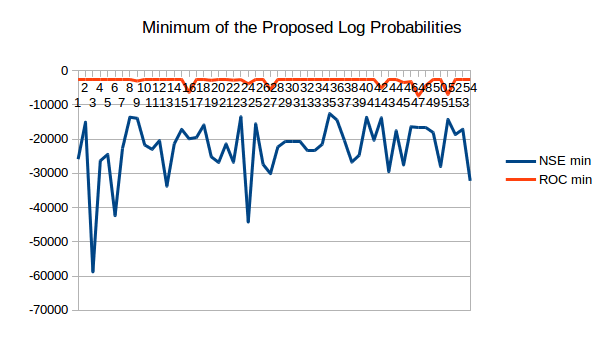
\includegraphics{data/minROCvNSE.png}
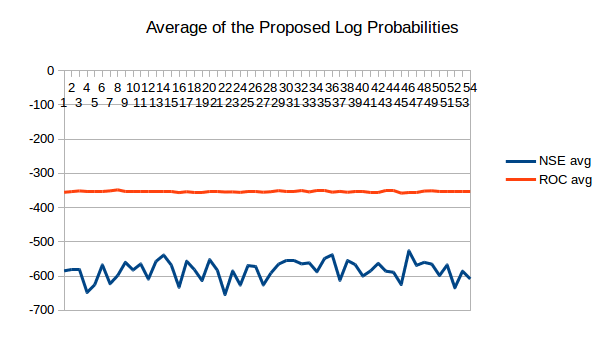
\includegraphics{data/avgROCvNSE.png}
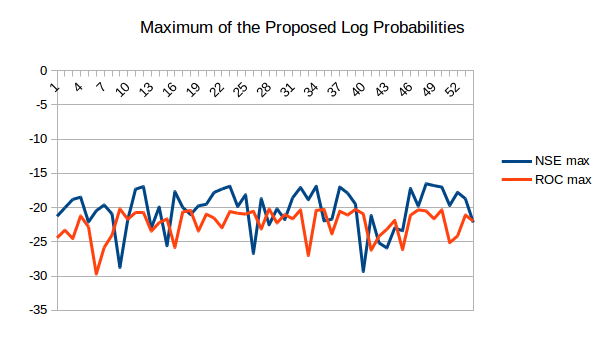
\includegraphics{data/maxROCvNSE.png}

\subsubsection{Use Sections of the Simulated Yeast Genome}

See cubfits/misc/S.cervisiae.REU13/random5ths.r


\subsubsection{If possible, NSE Patch}

One option to look into is to drop lp\_c\_raw from the code, and use rowsums like the Roc model. The two problems with that are that, as far as I can tell, lp.c.raw actually fixes the error in some cases, and using yaa * lp.vec complains for the NSE code. Not sure.

\subsubsection{Look into an R Vim extension or RStudio}

RStudio installed (also CMake), and it's VERY nice. Very intuitive, good use of screen real estate, and it holds a lot of information that I need at once. It keeps launching into /home/lbrown/PACKAGES/rstudio/bin though.

\subsubsection{Debugging Thoughts}

This was in last weeks summary, but it's included here for completeness.

How to GDB an R session
\begin{enumerate}
\item cd /home/lbrown/cubfits/misc/R
\item R -d gdb
\item run
\item source("debug\_nsef.r")
\item Ctrl-C
\item continue
\end{enumerate}





\subsection{Goals for next Week}
\begin{enumerate}
\item NSE Run Sections of Simulated Yeast Geome
\item Find out what causes some of the probabilties to go outrageously high
\item Compare Min, Max, and Average Values
\item Use Sections of the Simulated Yeast Genome
\item More information on Codon Position
\item Look into an R Vim extension or RStudio
\item Debugging Thoughts
\end{enumerate}


\end{document} %End of day document, REMOVE
